%!TEX root = ../msc_thesis.tex

\begin{appendices}


%%%%%%%%%%%%%%%%%%%%%%%%%%%%%%%%%%%%%%%%%%%%%%%%%%%%%%%%%%%%%%%%%%%%%%%%%%%%%%%%%%%%%%%%%%
%%%%%%%%%%%%%%%%%%%%%%%%%%%%%%%%%%%%%%%%%%%%%%%%%%%%%%%%%%%%%%%%%%%%%%%%%%%%%%%%%%%%%%%%%%
%%% Loss function optimization
%%%%%%%%%%%%%%%%%%%%%%%%%%%%%%%%%%%%%%%%%%%%%%%%%%%%%%%%%%%%%%%%%%%%%%%%%%%%%%%%%%%%%%%%%%
%%%%%%%%%%%%%%%%%%%%%%%%%%%%%%%%%%%%%%%%%%%%%%%%%%%%%%%%%%%%%%%%%%%%%%%%%%%%%%%%%%%%%%%%%%

\chapter{Loss function optimization}
\label{ch:appendix_loss_func_opt}

As mentioned before, in machine learning the goal is to find the parameters that minimize a loss function such as the one in equation \eqref{eq:logistic_example_loss_function}. In some cases like linear regression, it is possible to use the first and second order conditions to find a closed formula to find the parameters; but in many other cases this cannot be done, like in logistic regression, so we resort to numerical optimization techniques. The general problem of unconstrained optimization \cite{nocedal2006numerical} is
\begin{equation}
  \min_{\boldsymbol{\theta} \in \mathbb{R}^p} L(\boldsymbol{\theta}).
\end{equation}

In machine learning, $L$ is usually a convex loss function and $\boldsymbol{\theta}$ is a parameter or vector of parameters. A solution is a vector $\boldsymbol{\theta}^*$ called local minimizer, which minimizes the function $L$ in a neighborhood around $\boldsymbol{\theta}^*$. Formally, a vector $\boldsymbol{\theta}^*$ is a local minimizer if there exists a neighborhood $\mathcal{V}$ of $\boldsymbol{\theta}^*$ such that $L(\boldsymbol{\theta}^*) \leq L(\boldsymbol{\theta})$ for all $\boldsymbol{\theta} \in \mathcal{V}$.

The sufficient second order conditions are used in numerical optimization. Suppose that the Hessian matrix $\nabla^2 L$ is continuous in an open neighborhood of $\boldsymbol{\theta}^*$, that the gradient $\nabla L(\boldsymbol{\theta}^*) = 0$ and that $\nabla^2 L(\boldsymbol{\theta}^*)$ is positive definite; then $\boldsymbol{\theta}^*$ is a local minimizer of $L$. In general, all algorithms search for a point $\boldsymbol{\theta}^*$ such that $\nabla L(\boldsymbol{\theta}^*) = 0$ \cite{nocedal2006numerical}.

Many numerical optimization algorithms are iterative, such as coordinate descent, Newton and quasi-Newton methods, gradient free methods, and gradient descent. Coordinate descent algorithms work by fixing all but one parameter in each iteration and then minimizing the loss function with respect to the remaining parameter \cite{friedman2007pathwise, wright2015coordinate}.
Newton methods use a second-order Taylor series approximation to the loss function and iteratively descend by computing the Hessian matrix \cite[p.~22]{nocedal2006numerical}. Quasi-Newton methods use this same idea, but instead of computing the Hessian matrix exactly, they use some approximation to it \cite{byrd1995limited} \cite[p.~23]{nocedal2006numerical}.
Gradient free algorithms are used when the gradient of the loss function is not available, which could be for computational reasons, for unavailability, or practical reasons \cite{rios2013derivative}. They include simulated annealing, swarm algorithms and genetic algorithms.
Gradient descent is explained in the next subsection.

\subsection{Gradient descent (GD)}

Gradient descent belongs to a family of optimization algorithms called \textbf{line search algorithms}. In each iteration, these algorithms search for a direction in which to move and then update the current value in accordance to that direction \cite[p.~19]{nocedal2006numerical}. That is, in the $k$-th iteration, $\boldsymbol{\theta}$ has the value $\boldsymbol{\theta}_k$, and the algorithms look for a direction $\boldsymbol{p}_k$ to update to a new value $\boldsymbol{\theta}_{k+1} = \boldsymbol{\theta}_k + \alpha_k \boldsymbol{p}_k$, where $\alpha_k > 0$ is the ``distance'' in which the algorithm moves toward direction $\boldsymbol{p}_k$, and is called \textbf{step length}. Once that the value of the parameter is updated, the algorithm finds a new direction in which to move forward and then updates the parameter value again. This is done until a stopping criterion is met. This usually is that the gradient vector norm is smaller than a certain small positive scalar.

In gradient descent, the direction $\boldsymbol{p}_k$ in which the algorithm moves is the maximum descent direction, that is, the negative of the gradient $-\nabla L(\boldsymbol{\theta}_k)$. So, in each iteration $\boldsymbol{\theta}$ is updated as such
\begin{equation}
  \label{eq:parameter_update_gd}
  \boldsymbol{\theta}_{k+1} = \boldsymbol{\theta}_k - \alpha_k \nabla L(\boldsymbol{\theta}_k).
\end{equation}

Choosing the step length $\alpha_k$ is problematic because it is desirable to find a value such that the function $L$ decreases as much as possible, but it is not desirable to spend too much time choosing the value. The best option is the global minimizer of the auxiliary function $\phi(\alpha_k) = L(\boldsymbol{\theta}_k + \alpha_k \boldsymbol{p}_k)$, but it may be too expensive to compute \cite[p.~31]{nocedal2006numerical}. Generally, heuristics are used to choose the sequence of values for $\alpha_k$ and try which one satisfies those conditions. One of those conditions is called Armijo conditions, and finds the $\alpha_k$ that allows a sufficient descent in the function $L$, measured as
\begin{equation}
    L(\boldsymbol{\theta}_k + \alpha_k \boldsymbol{p}_k) \leq L(\boldsymbol{\theta}_k) + c_1 \alpha_k \nabla L(\boldsymbol{\theta}_k)^T \boldsymbol{p}_k,
\end{equation}
for a constant $c_1 \in (0, 1)$. Usually $c_1$ is small, such as $10^{-4}$. This condition may not be enough, because for very small values of $\alpha_k$ the condition can be met, and very small step lengths are not always desirable. One way to fix this is to use backtracking, which consists in choosing a big value of $\alpha_k$ (such as $\alpha_k = 1$), and then an iterative sub-algorithm is initiated to decrease the value of $\alpha_k$ until the Armijo condition is met. Another way to choose the step length $\alpha_k$ is using the outer product of the gradient with itself, as shown in \cite{duchi2011adaptive}.

In the following paragraphs, an example of logistic regression is shown to understand how gradient descent works.

The loss function to be minimized, defined in equation \eqref{eq:logistic_example_loss_function}, is
\begin{equation}
  \begin{split}
    L(\boldsymbol{\theta}) & = - \sum_{i=1}^{n} \left[ y_i \log(\sigma(\boldsymbol{\theta}^T \boldsymbol{x_i})) + (1-y_i) \log(1-\sigma(\boldsymbol{\theta}^T \boldsymbol{x_i})) \right] \\
    & = - \sum_{i=1}^{n}{\ell_i(\boldsymbol{\theta})}
  \end{split}
\end{equation}
where $\sigma(\cdot)$ is the logistic sigmoid function, $\boldsymbol{\theta}^T \boldsymbol{x_i} = \sum_{j=0}^{p}{\theta_j x_{ij}}$, $x_{i1} = 1$ for all $i \in \left\{1, ..., n \right\}$ and $\ell_i(\boldsymbol{\theta})$ is defined as
\begin{equation}
  \ell_i(\boldsymbol{\theta}) = y_i \log(\sigma(\boldsymbol{\theta}^T \boldsymbol{x_i})) + (1-y_i) \log(1-\sigma(\boldsymbol{\theta}^T \boldsymbol{x_i})).
\end{equation}

Taking the partial derivatives of the loss function with respect to the parameters the result is
\begin{equation}
  \frac{\partial L}{\partial \theta_j} = - \sum_{i = 1}^n { \frac{\partial \ell_i}{\partial \theta_j} }
\end{equation}
and, using the fact that $\sigma'(w) = \sigma(w)(1-\sigma(w))$, then each partial derivative from the sum
\begin{equation}
  \begin{split}
    \frac{\partial \ell_i}{\partial \theta_j} & =
    \frac{y_i \sigma'(\boldsymbol{\theta}^T \boldsymbol{x_i}) x_{ij} }  {\sigma(\boldsymbol{\theta}^T \boldsymbol{x_i})} + \frac{(1 - y_i) (-1) \sigma'(\boldsymbol{\theta}^T \boldsymbol{x_i}) x_{ij}} {1 - \sigma(\boldsymbol{\theta}^T \boldsymbol{x_i})} \\
    & = \frac{\sigma'(\boldsymbol{\theta}^T \boldsymbol{x_i}) x_{ij} y_i}{\sigma(\boldsymbol{\theta}^T \boldsymbol{x_i})} - \frac{(1 - y_i) \sigma'(\boldsymbol{\theta}^T \boldsymbol{x_i}) x_{ij}}{1 - \sigma((\boldsymbol{\theta}^T \boldsymbol{x_i}))} \\
    & = \sigma'(\boldsymbol{\theta}^T \boldsymbol{x_i}) x_{ij} \left(\frac{y_i}{\sigma(\boldsymbol{\theta}^T \boldsymbol{x_i})} - \frac{1-y_i}{1-\sigma(\boldsymbol{\theta}^T \boldsymbol{x_i})} \right) \\
    & = \sigma'(\boldsymbol{\theta}^T \boldsymbol{x_i}) x_{ij} \left(\frac{y_i - y_i \sigma(\boldsymbol{\theta}^T \boldsymbol{x_i}) -
    \sigma(\boldsymbol{\theta}^T \boldsymbol{x_i}) + y_i \sigma(\boldsymbol{\theta}^T \boldsymbol{x_i})}{\sigma(\boldsymbol{\theta}^T \boldsymbol{x_i})(1-\sigma(\boldsymbol{\theta}^T \boldsymbol{x_i}))} \right) \\
    & = x_{ij}(y_i - \sigma(\boldsymbol{\theta}^T \boldsymbol{x_i})).
  \end{split}
\end{equation}

Finally, the partial derivative is
\begin{equation}
  \frac{\partial L}{\partial \theta_j} = - \sum_{i = 1}^n { x_{ij}(y_i - \sigma(\sum_{j=0}^{p}{\theta_j x_{ij}})) }.
\end{equation}

Hence, the gradient descent direction for each iteration is
\begin{equation}
  \nabla_{\boldsymbol{\theta}} L = \left( \frac{\partial L}{\partial \theta_1}, ..., \frac{\partial L}{\partial \theta_p} \right)^T.
\end{equation}

To minimize the loss function, an initial vector of parameters $\boldsymbol{\theta}^0 \in \mathbb{R}^p$ is chosen, and in each iteration this vector is updated using equation \eqref{eq:parameter_update_gd} until certain criteria are met.

This algorithm was implemented in the R programming language \cite{R_manual} by generating a data matrix $\boldsymbol{X} \in \mathbb{R}^{n \times 1}$ with $n = 1000$ such that $\boldsymbol{x_i} \sim N(0, 1)$ for each $i \in \left\{1, ..., n \right\}$.
Then an auxiliary vector was computed, $p_i = \frac{1}{1 + \exp \left( - \theta_0 - \theta_1 x_i^{(1)} \right)}$, with $\theta_0 = -5$ and $\theta_1 = 5$. Finally, the response variable $\boldsymbol{y}$ was built simulating Bernoulli random variables, such that $y_i \sim \mathrm{Bern}(p_i)$.
The implementation is compared with the result of the \texttt{glm} package.

The initial vector of parameters was $\boldsymbol{\theta}^0 = (0, 0)^T$ and a constant value of $\alpha_k = 0.1$ was used. The stopping criterion was that the norm of the gradient, i.e. $\norm{\nabla_{\boldsymbol{\theta}} L(\boldsymbol{\theta})}$, should be less than $10^{-8}$, this being the approximate square root of the double-precision floating-point format; or that the norm of the difference of the parameters from one iteration to the other, i.e. $\norm{\boldsymbol{\theta}_{k+1} - \boldsymbol{\theta}_k}$, should be less than $10^{-8}$. This was achieved after \numprint{3704} iterations.

Figure \ref{fig:GD_plots} shows the results of the implementation. On the left, the value of the loss function in each iteration can be seen. On the right, the parameter vector's value in each iteration. The red dot is the value of the estimate by the \texttt{glm} package. It can be seen that the implemented algorithm converges to this value.

\begin{figure}[H]
    \centering
    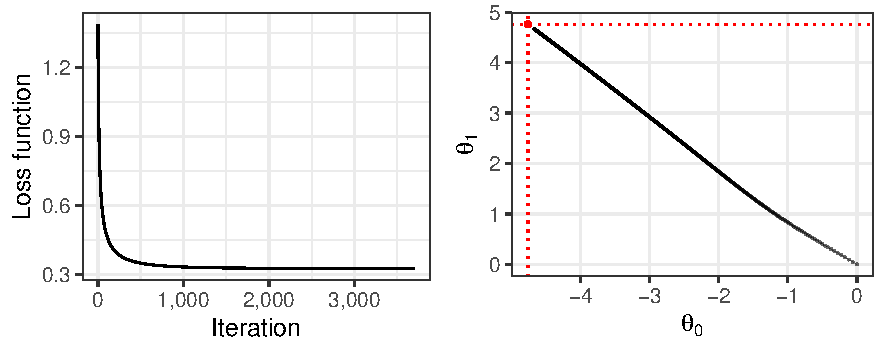
\includegraphics[width=\textwidth]{GD_plots}
    \caption{Example of gradient descent for logistic regression.}
    \label{fig:GD_plots}
\end{figure}

\subsection{Stochastic gradient descent (SGD)}

In machine learning it is common to assume that observations are independent and identically distributed, thus, it is also common to find the need to solve optimization problems of the form
\begin{equation}
  \min_{\boldsymbol{\theta} \in \mathbb{R}^p} L(\boldsymbol{\theta}), \quad \text{with} \, \,
  L(\boldsymbol{\theta}) = \frac{1}{n} \sum_{i = 1}^n { \ell_i(\boldsymbol{\theta}) }.
\end{equation}

That is, the loss function that needs to be minimized is usually a sum or average of several indexed functions in which each indexed function depends only on one observation of the data set. For example, in logistic regression, the loss function that is expressed in that way.

Gradient descent uses iterations in the form
\begin{equation}
  \boldsymbol{\theta}_{k+1} = \boldsymbol{\theta}_k - \alpha_k \nabla L(\boldsymbol{\theta}_k) :=\boldsymbol{\theta}_k - \frac{\alpha_k}{n} \sum_{i = 1}^n \nabla \ell_i(\boldsymbol{\theta}_k),
\end{equation}
which involves evaluating $n$ gradients (one for each observation) and then taking an average. In some cases of machine learning, $n$ can be really big; hence computing all of those gradients in each iteration is expensive. That is why methods such as SGD are used, in which the number of gradients to compute does not depend on $n$ but instead it is constant. SGD uses iterations of the form
\begin{equation}
  \boldsymbol{\theta}_{k+1} = \boldsymbol{\theta}_k - \alpha_k \nabla \ell_{i_k}(\boldsymbol{\theta}_k),
\end{equation}
where $i_k \in \left\{1, 2, ..., n \right\}$ is randomly chosen. The gradient $\nabla \ell_{i_k}(\boldsymbol{\theta}_k)$ is an unbiased estimator of $\nabla L(\boldsymbol{\theta}_k)$. This way, each iteration is computationally inexpensive because it involves the computation of only one gradient.
It can happen that some $\nabla \ell_{i_k}(\boldsymbol{\theta}_k)$ in particular does not give a descent direction from $\boldsymbol{\theta}_k$, but on average they yield descent directions. Thus, the sequence $\left\{ \boldsymbol{\theta}_0, \boldsymbol{\theta}_1, ... \right\}$, under certain conditions, leads to a minimizer $\boldsymbol{\theta}^*$.

\subsection{Mini-batch gradient descent}

An approach that lies between the two extremes of computing the gradients of all observations and the gradient of just one observation is \textbf{mini-batch gradient descent}. In mini-batch gradient descent, one chooses a fixed integer $l$, then the data set is divided in batches of size $l$, where the values in each batch are randomly chosen. Then, each of these batches is used to compute the gradient and update the values of the parameters. Usually $l$ is a small number compared to the size of the data set, but big enough so that the gradient estimation is not too noisy, such as $l = 32$ or $l = 100$. This way, each iteration is cheaper because it involves the computation of only $l$ gradients instead of $n$, with $l << n$. Stochastic gradient descent (SGD) is just mini-batch gradient descent with $l = 1$.

So, mini-batch gradient descent updates the value of the parameters in each iteration as such
\begin{equation}
  \boldsymbol{\theta}_{k+1} = \boldsymbol{\theta}_k - \frac{\alpha_k}{n} \sum_{i = 1}^l \nabla \ell_i(\boldsymbol{\theta}_k).
\end{equation}

We implemented mini-batch gradient descent for logistic regression in R and test it with the same simulated data set as in the previous example. Figure \ref{fig:Mini-batch_GD_plots} shows the results of the implementation. Each of the plots shows the values of the parameters in each iteration, but the difference in each plot is the size of the mini-batch $l$. It is clear that with bigger $l$, the descent directions are less noisy, but in the end they all converge to more or less the same value.

\begin{figure}[H]
    \centering
    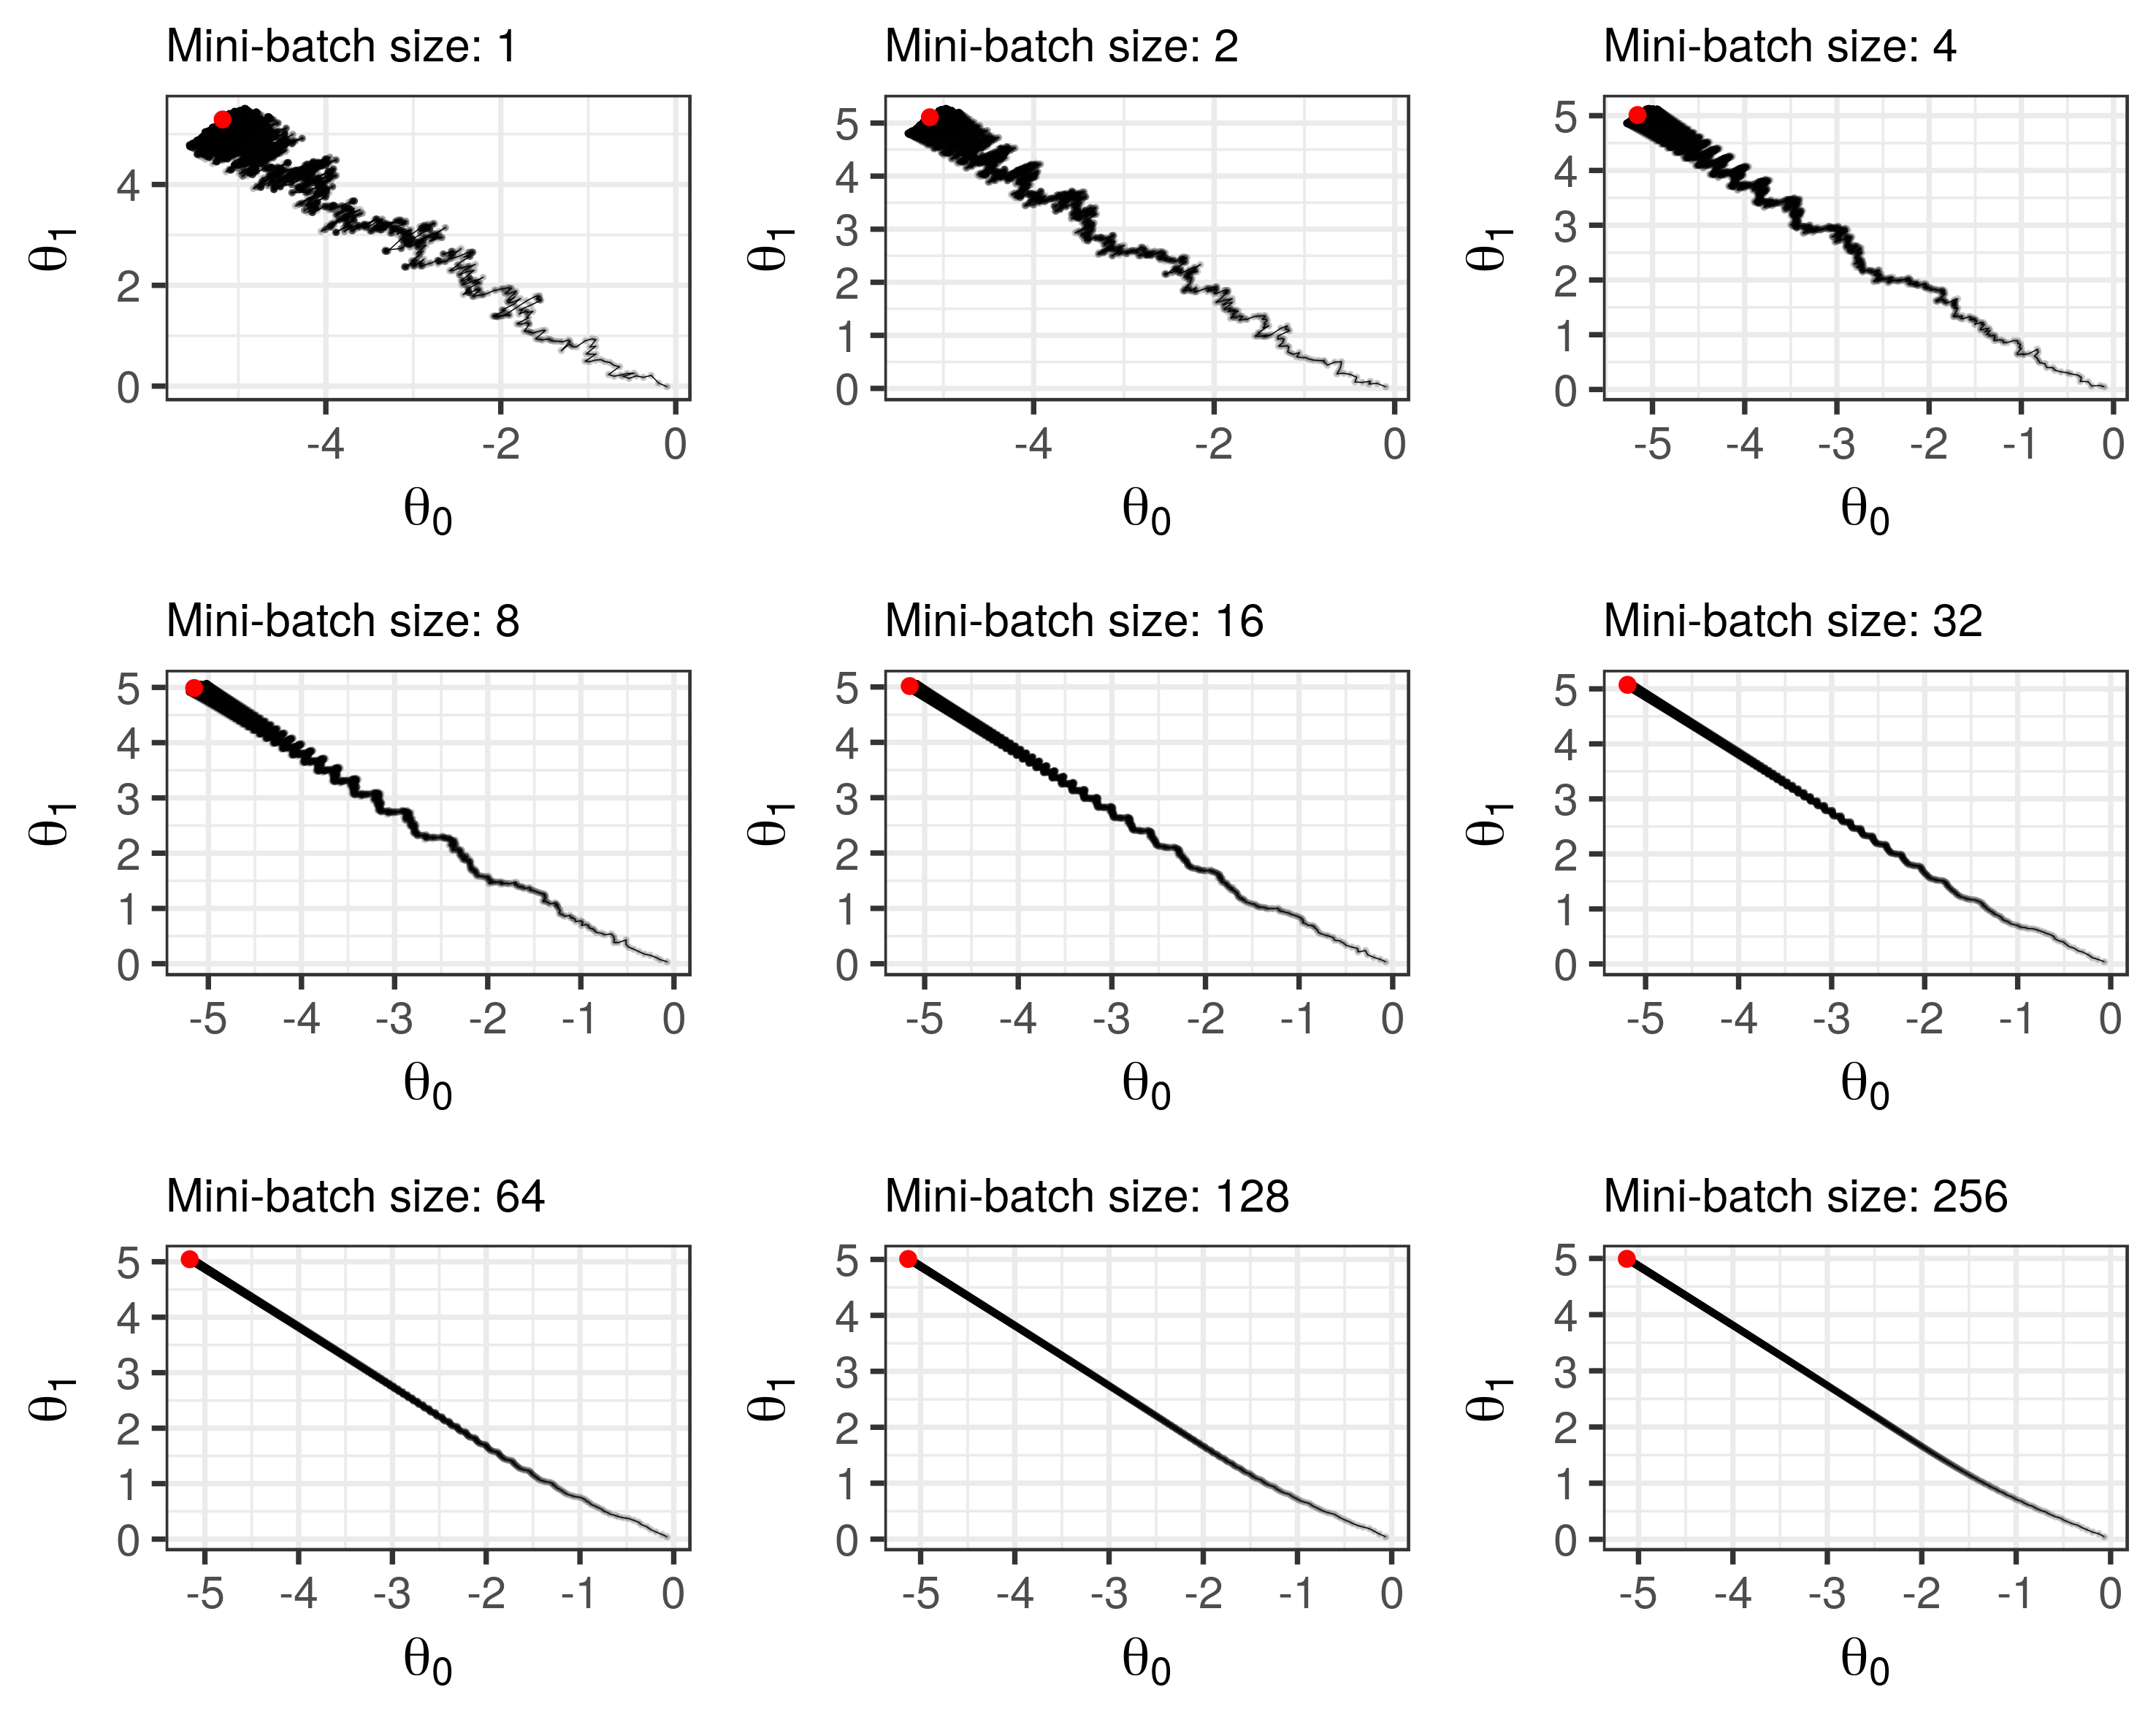
\includegraphics[width=\textwidth]{Mini-batch_GD_plots.png}
    \caption{Example of mini-batch gradient descent for logistic regression comparing mini-batch sizes.}
    \label{fig:Mini-batch_GD_plots}
\end{figure}








%%%%%%%%%%%%%%%%%%%%%%%%%%%%%%%%%%%%%%%%%%%%%%%%%%%%%%%%%%%%%%%%%%%%%%%%%%%%%%%%%%%%%%%%%%
%%%%%%%%%%%%%%%%%%%%%%%%%%%%%%%%%%%%%%%%%%%%%%%%%%%%%%%%%%%%%%%%%%%%%%%%%%%%%%%%%%%%%%%%%%
%%% Highest uncertainty images
%%%%%%%%%%%%%%%%%%%%%%%%%%%%%%%%%%%%%%%%%%%%%%%%%%%%%%%%%%%%%%%%%%%%%%%%%%%%%%%%%%%%%%%%%%
%%%%%%%%%%%%%%%%%%%%%%%%%%%%%%%%%%%%%%%%%%%%%%%%%%%%%%%%%%%%%%%%%%%%%%%%%%%%%%%%%%%%%%%%%%

\chapter{Images with highest uncertainty}
\label{ch:appendix_loss_func_opt_images_high_uncertainty}

Figures \ref{fig:MNIST_high_uncertainty_examples}, \ref{fig:cats_dogs_high_uncertainty_examples} and \ref{fig:CIFAR10_high_uncertainty_examples} show the most uncertain examples for a Bayesian CNN using the variation ratios acquisition function with the MNIST, cats and dogs, and CIFAR10 datasets, respectively.

In the case of the MNIST and cats and dogs datasets, some unusual examples can be seen. For instance, in the case of the third row and first column of figure \ref{fig:MNIST_high_uncertainty_examples}, it is not clear what number it is. The same happens with the ninth row and second column. In figure \ref{fig:cats_dogs_high_uncertainty_examples}, the element in the second row and second column is a cat on books in a book-shelf, but it is not clear at first glance. And the picture in the fourth row and fourth column is peculiar because it has a star shape. On the contrary to the previous two datasets, in the case of the cats and dogs dataset, figure \ref{fig:CIFAR10_high_uncertainty_examples} does not show any obvious deviation from the rule.
% Nevertheless, the CIFAR10 is a harder problem to solve than the cats and dogs problem because there are ten classes in which to classify instead of two.

\begin{figure}[H]
    \centering
    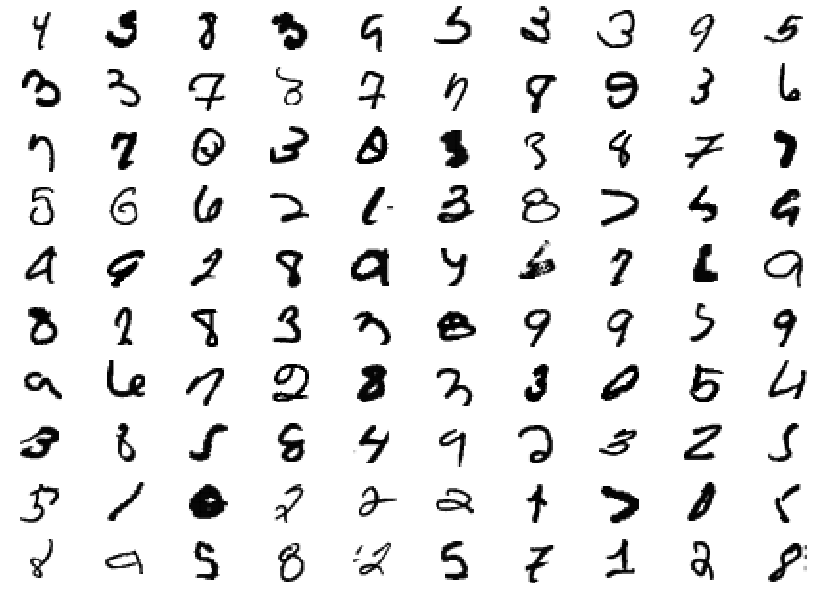
\includegraphics[width=\textwidth]{MNIST_high_uncertainty_examples}
    \caption{Images with highest uncertainties in the MNIST dataset.}
    \label{fig:MNIST_high_uncertainty_examples}
\end{figure}


\begin{figure}[H]
    \centering
    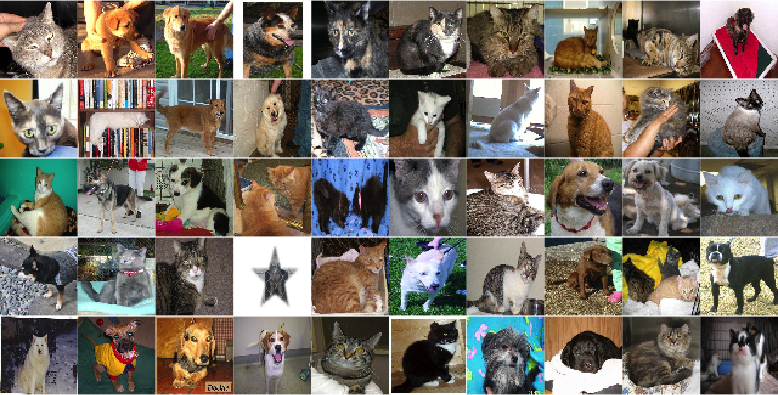
\includegraphics[width=\textwidth]{cats_dogs_high_uncertainty_examples}
    \caption{Images with highest uncertainties in the cats and dogs dataset.}
    \label{fig:cats_dogs_high_uncertainty_examples}
\end{figure}


\begin{figure}[H]
    \centering
    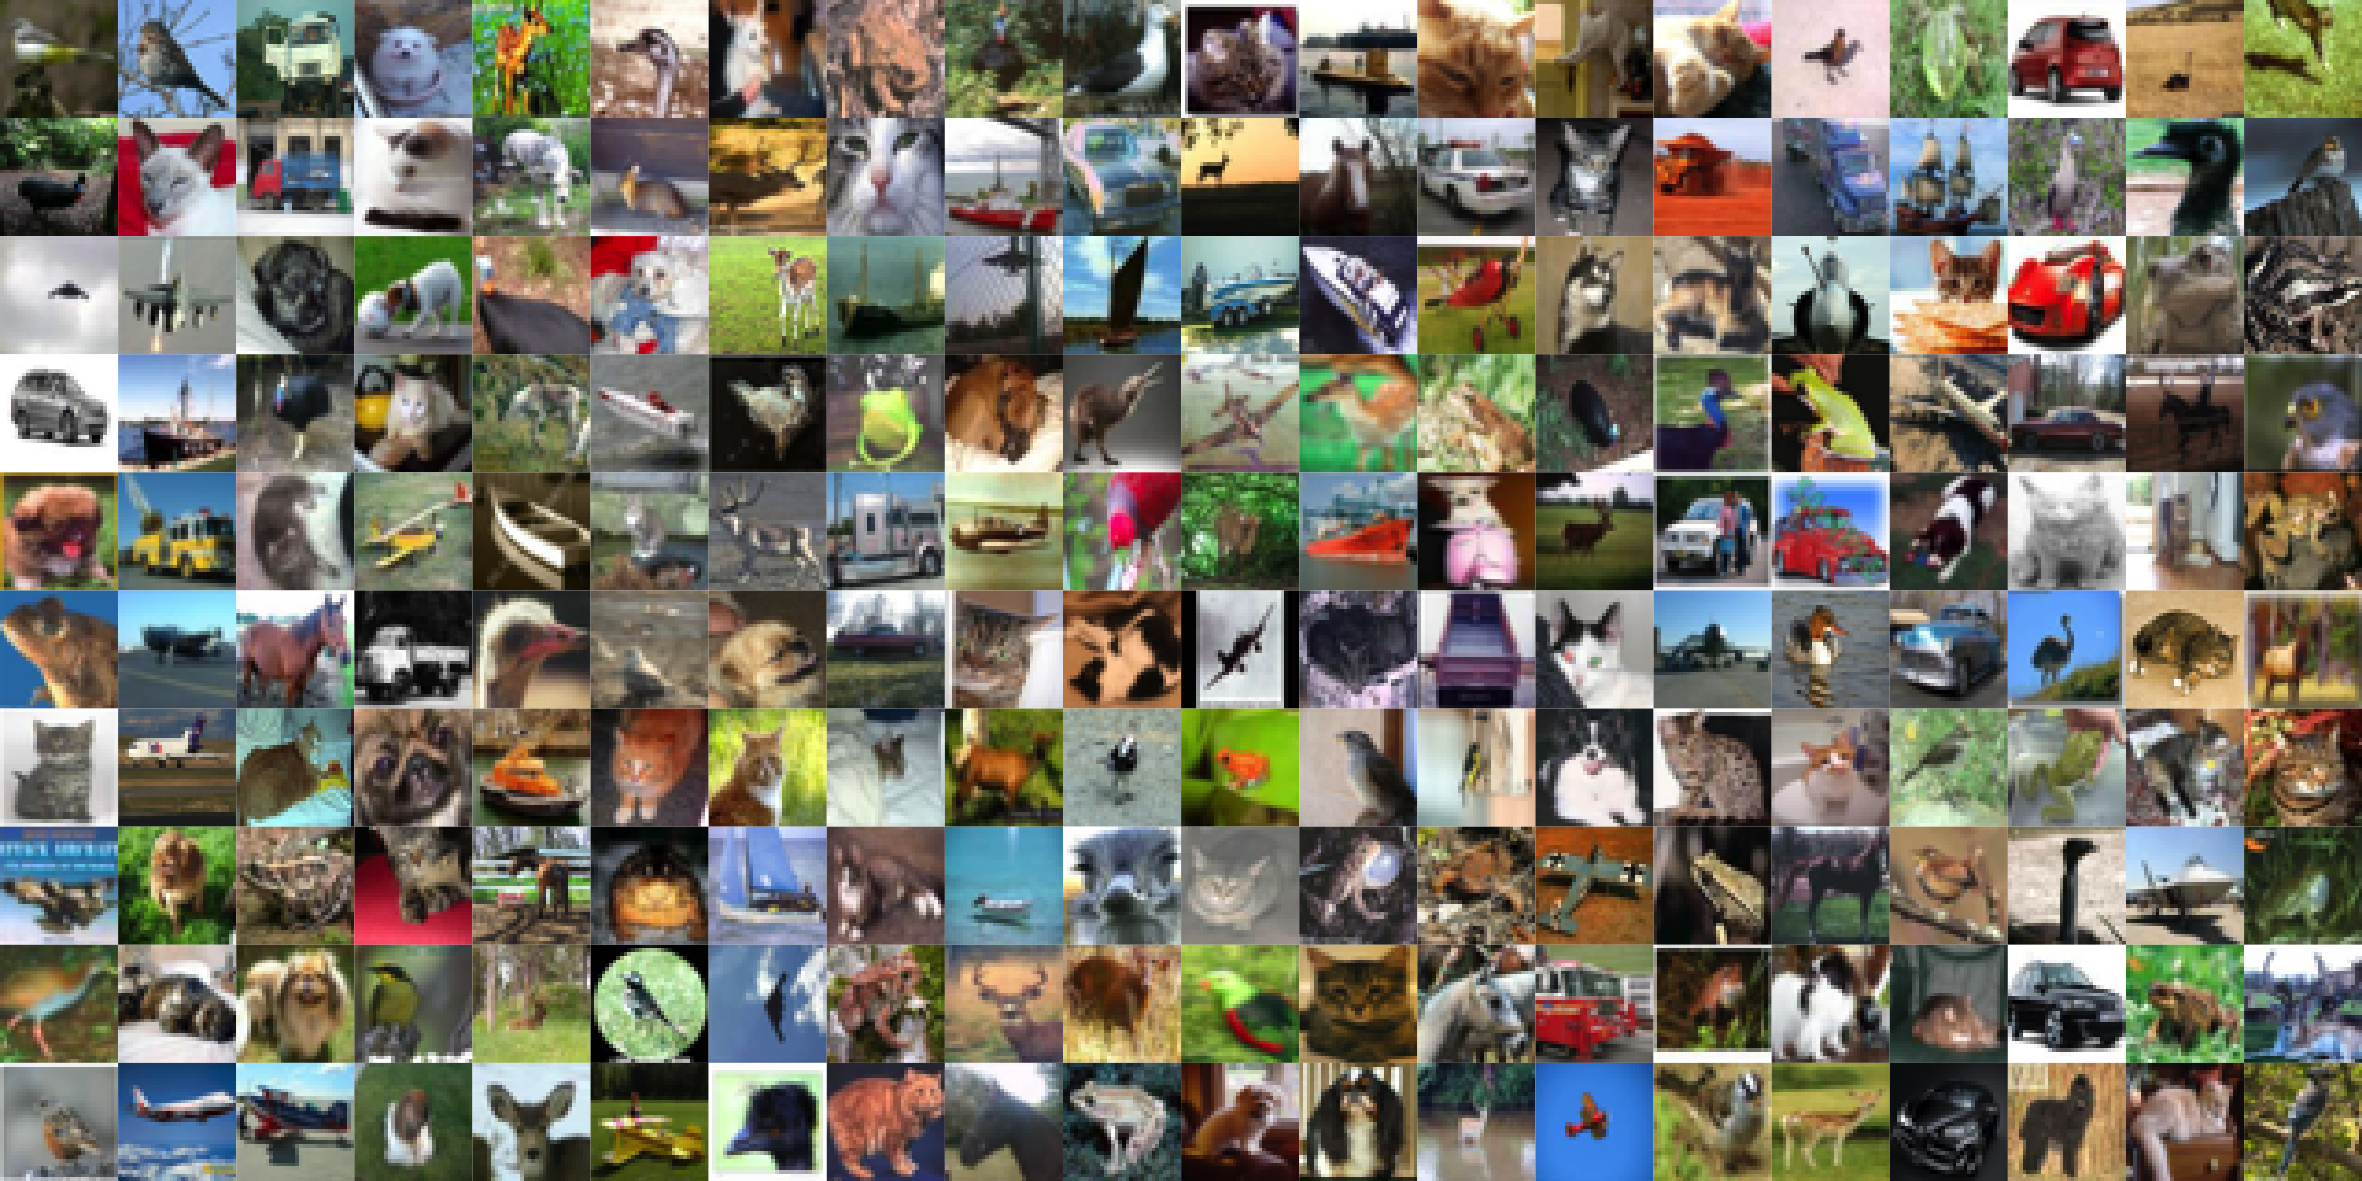
\includegraphics[width=\textwidth]{CIFAR10_high_uncertainty_examples}
    \caption{Images with highest uncertainties in the CIFAR10 dataset.}
    \label{fig:CIFAR10_high_uncertainty_examples}
\end{figure}





\end{appendices}
